\subsection{Insegnante}

\subsubsection{Panoramica insegnante}
\begin{figure}[H]
\centering
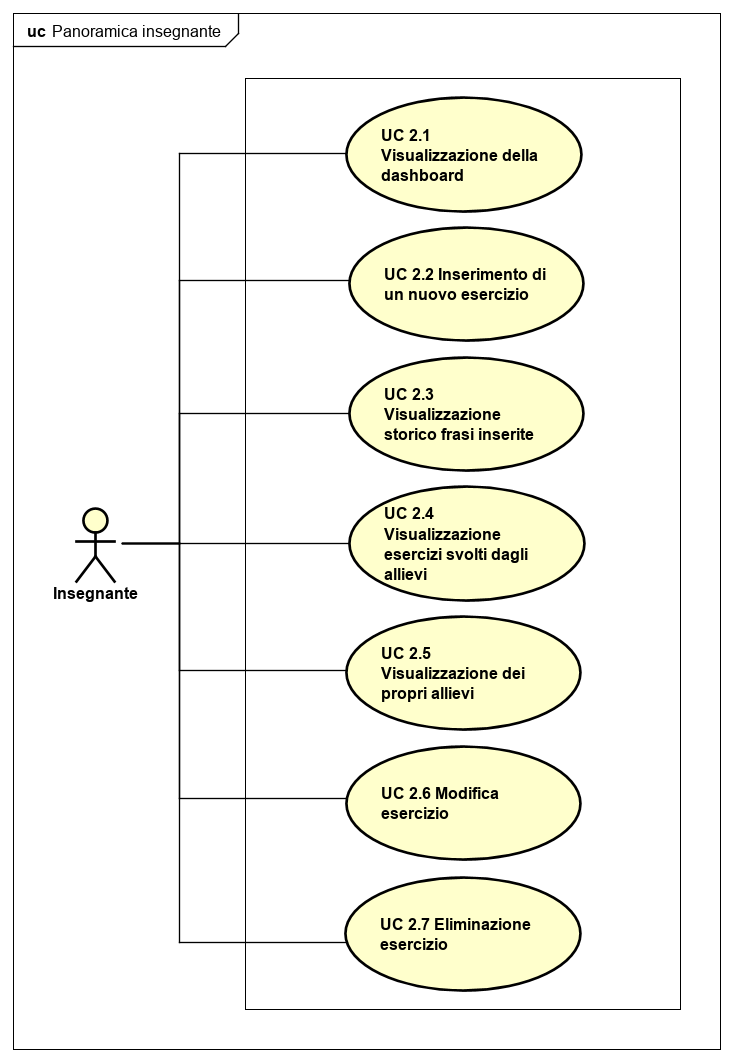
\includegraphics[width=17cm, height=20cm]{img/PanoramicaInsegnanti.png} 
\caption{Panoramica insegnante}
\end{figure}

\subsubsection{UC 2.1 Visualizzazione della dashboard}
\begin{itemize}
	\item[•] \textbf{Attori}: Insegnante;
	\item[•] \textbf{Descrizione}: l’insegnante accede alla propria dashboard dove può vedere i suoi dati, le frasi che ha assegnato agli alunni, il numero e i nomi degli studenti che possiede. Può effettuare modifiche agli esercizi e ai suoi dati personali.
	\item[•] \textbf{Precondizione}: l'insegnante si è autenticato;
	\item[•] \textbf{Postcondizione}: l'insegnante visualizza il profilo personale e il numero di allievi, le frasi che ha inserito, i suoi dati e le soluzioni spedite dagli allievi.
	\item[•] \textbf{Flusso degli eventi}: l'insegnante si è autenticato correttamente nel sistema. 

\end{itemize}

\subsubsection{UC 2.2 Inserimento di un nuovo esercizio}
\begin{figure}[H]
	\centering
	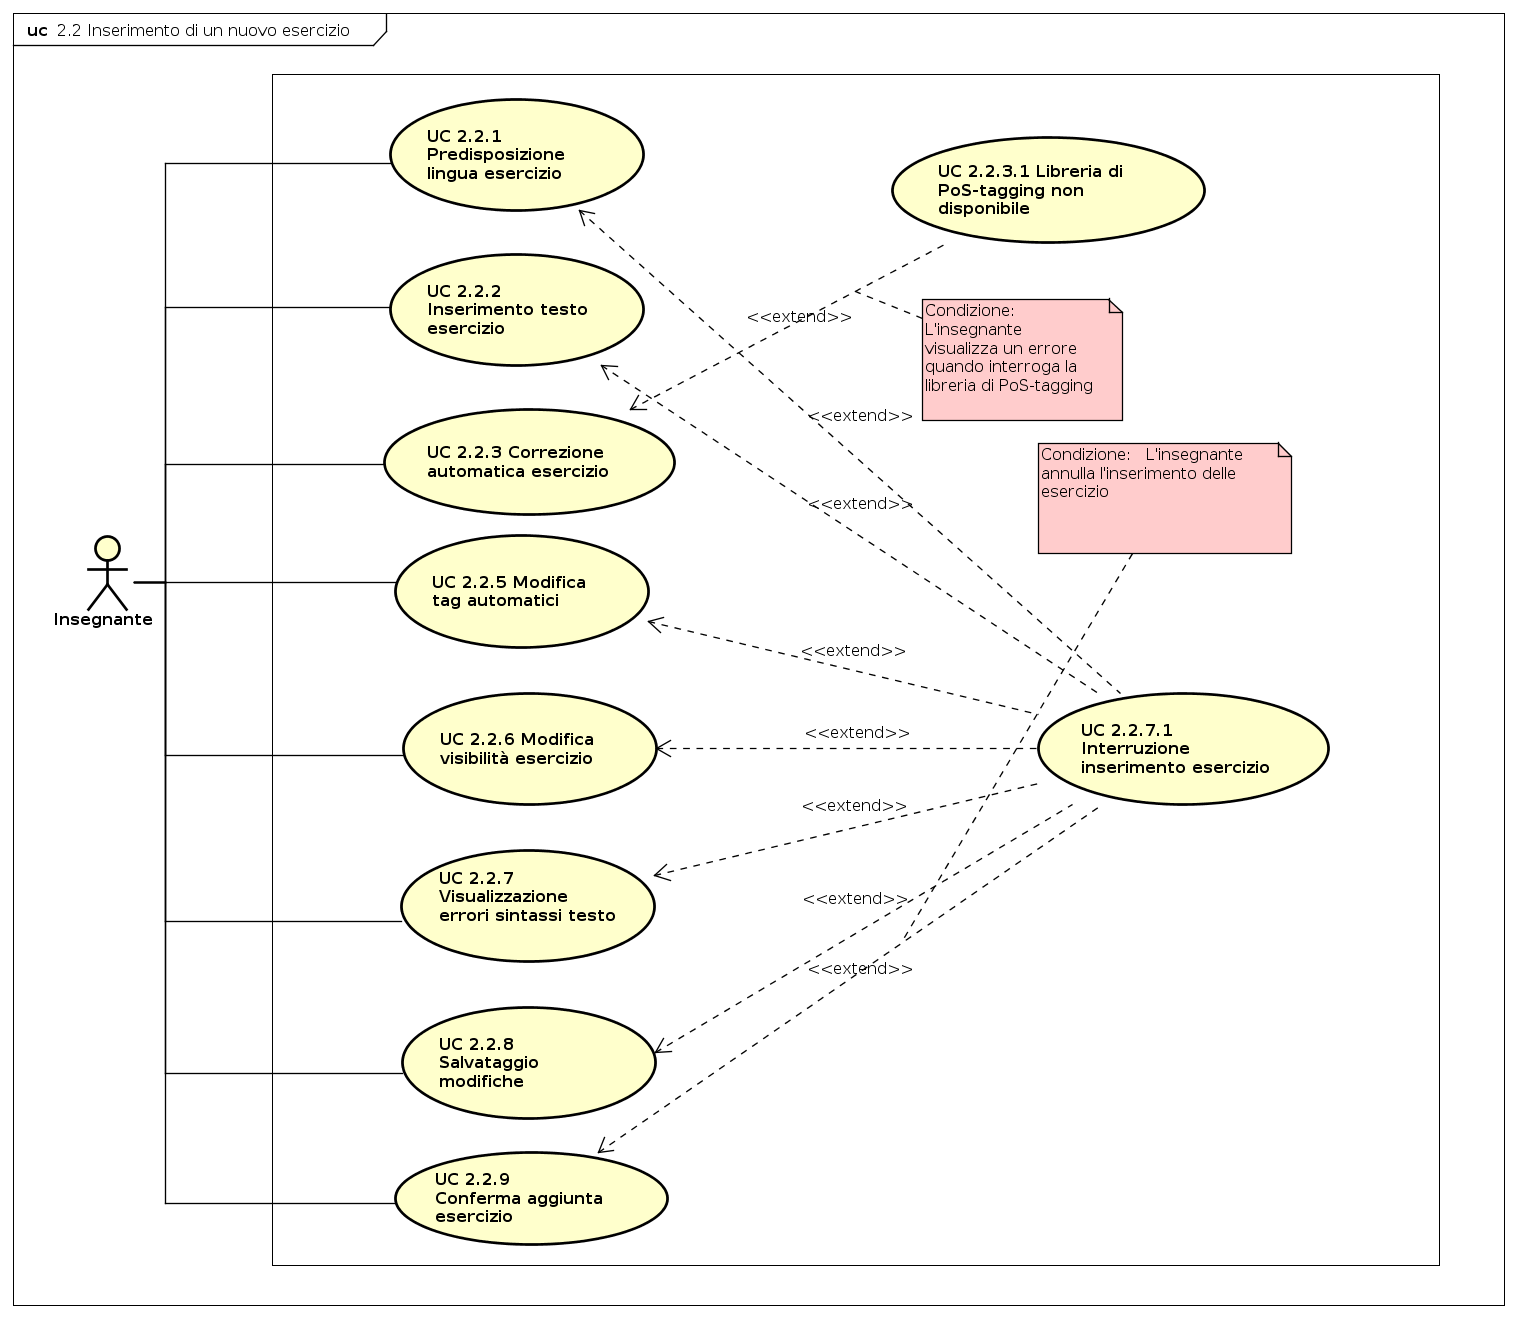
\includegraphics[width=17cm]{img/UC22.png} 
	\caption{Caso d'uso UC 2.2;}
\end{figure}


\begin{itemize}
	\item[•] \textbf{Attori}: Insegnante;
	\item[•] \textbf{Descrizione}: l'insegnante aggiunge un nuovo esercizio e può scegliere la lingua, scrivere il testo,
modificare i tag automatici ecc. Potrà poi confermare l'aggiunta dell'esercizio;
	\item[•] \textbf{Precondizione}: l'insegnante si è autenticato e visualizza il proprio profilo personale;
	\item[•] \textbf{Postcondizione}: l'insegnante ha inserito un esercizio;
	\item[•] \textbf{Flusso degli eventi}:
	\begin{enumerate}
		\item UC 2.2.1 Predisposizione lingua esercizio;
		\item UC 2.2.2 Inserimento testo esercizio;
		\item UC 2.2.3 Correzione automatica esercizio
		\item UC 2.2.5 Modifica tag automatici;
		\item UC 2.2.6 Modifica visibilità esercizio;
		\item UC 2.2.7 Visualizzazione errori sintassi testo;
		\item UC 2.2.8 Salvataggio modifiche;
		\item UC 2.2.9 Conferma aggiunta esercizio.
	\end{enumerate}
	\item[•] \textbf{Estensioni}:	
	\begin{enumerate}
		\item UC 2.2.3.1 Libreria di PoS-tagging non disponibile
		\item UC 2.2.7.1 Interruzione inserimento esercizio.
	\end{enumerate}
	\item[•] \textbf{Flusso degli eventi alternativo}:
	\begin{enumerate}
		\item UC 2.2.4 Inserimento soluzione alternativa.
	\end{enumerate}
\end{itemize}

\subsubsection{UC 2.2.1 Predisposizione lingua esercizio}
\begin{itemize}
	\item[•] \textbf{Attori}: Insegnante;
	\item[•] \textbf{Descrizione}: l'insegnante sceglie la lingua dell’esercizio che vuole scrivere;
	\item[•] \textbf{Precondizione}: l'insegnante sta inserendo un esercizio;
	\item[•] \textbf{Postcondizione}: l'insegnante ha scelto la lingua dell'esercizio;
	\item[•] \textbf{Flusso degli eventi}: l'insegnante ha iniziato la procedura di inserimento di un esercizio all'interno del suo profilo personale.
\end{itemize}

\subsubsection{UC 2.2.2 Inserimento testo esercizio}
\begin{itemize}
	\item[•] \textbf{Attori}: Insegnante;
	\item[•] \textbf{Descrizione}: l'insegnante scrive il testo dell’esercizio;
	\item[•] \textbf{Precondizione}: l'insegnante sta inserendo un esercizio;
	\item[•] \textbf{Postcondizione}: l'insegnante ha inserito il testo dell'esercizio;
	\item[•] \textbf{Flusso degli eventi}: l'insegnante ha iniziato la procedura di inserimento esercizio e ha predisposto la lingua.
\end{itemize}


\subsubsection{UC 2.2.3 Correzione automatica esercizio}
\begin{itemize}
	\item[•] \textbf{Attori}: Insegnante, libreria di PoS-tagging;
	\item[•] \textbf{Descrizione}: l’insegnante ottiene automaticamente i tag dal testo dell’esercizio attraverso la libreria di PoS-tagging;
	\item[•] \textbf{Precondizione}: l'insegnante ha inserito il testo dell'esercizio;
	\item[•] \textbf{Postcondizione}: l'insegnante visualizza la soluzione dell'esercizio;
	\item[•] \textbf{Flusso degli eventi}: l'insegnante ha iniziato la procedura di inserimento esercizio, ha predisposto la lingua e inserito il testo. 
\end{itemize}

\subsubsection{UC 2.2.3.1 Libreria PoS-tagging non disponibile}
\begin{itemize}
	\item[•] \textbf{Attori}: Insegnante, Allievo;
	\item[•] \textbf{Descrizione}: L'attore rivece un messaggio di errore poichè la libreria di PoS-tagging non è disponibile; 
	\item[•] \textbf{Precondizione}: l'insegnante sta inserendo un esercizio o un  allievo sta svolgendo un esercizio;
	\item[•] \textbf{Postcondizione}: l'operazione viene interrotta;
	\item[•] \textbf{Flusso degli eventi}: l'insegnante ha iniziato la procedura di inserimento esercizio, ha predisposto la lingua e inserito il testo.
\end{itemize}


\subsubsection{UC 2.2.4 Inserimento soluzione alternativa}
\begin{itemize}
	\item[•] \textbf{Attori}: Insegnante;
	\item[•] \textbf{Descrizione}: l'insegnante, in caso di esercizi con più soluzioni, inserisce tag alternativi all’esercizio;
	\item[•] \textbf{Precondizione}: l'insegnante visualizza la soluzione dell'esercizio;
	\item[•] \textbf{Postcondizione}: l'insegnante aggiunge una soluzione alternativa;
	\item[•] \textbf{Flusso degli eventi}: l'insegnante ha iniziato la procedura di inserimento esercizio, ha predisposto la lingua, inserito il test e ricevuto una soluzione dalla libreria di PoS-tagging.
\end{itemize}


\subsubsection{UC 2.2.5 Modifica tag automatici}
\begin{itemize}
	\item[•] \textbf{Attori}: Insegnante, libreria di PoS-tagging;
	\item[•] \textbf{Descrizione}: l’insegnante modifica i tag generati automaticamente;
	\item[•] \textbf{Precondizione}: l'insegnante visualizza la soluzione dell'esercizio;
	\item[•] \textbf{Postcondizione}: l'insegnante ha modificato i tag generati automaticamente;
	\item[•] \textbf{Flusso degli eventi}: l'insegnante ha iniziato la procedura di inserimento esercizio, ha predisposto la lingua, inserito il testo e ricevuto una correzione automatica dalla libreria di PoS-tagging.
\end{itemize}

\subsubsection{UC 2.2.6 Modifica visibilità esercizio}
\begin{itemize}
	\item[•] \textbf{Attori}: Insegnante;
	\item[•] \textbf{Descrizione}: l'insegnante imposta la visibilità dell'esercizio, ovvero quali allievi possono visualizzarlo e sceglierlo;
	\item[•] \textbf{Precondizione}: l'insegnante sta inserendo un esercizio;
	\item[•] \textbf{Postcondizione}: l'insegnante ha modificato la visibilità dell'esercizio;
	\item[•] \textbf{Flusso degli eventi}: l'insegnante ha iniziato la procedura di inserimento esercizio, ha predisposto la lingua, inserito il testo, ricevuto una correzione automatica dalla libreria di PoS-tagging e modificato i tag automatici.
\end{itemize}

\subsubsection{UC 2.2.7 Visualizzazione errori sintassi testo}
\begin{itemize}
	\item[•] \textbf{Attori}: Insegnante;
	\item[•] \textbf{Descrizione}: l'insegnante visualizza gli errori relativi alla sintassi e la forma del testo che ha inserito;
	\item[•] \textbf{Precondizione}: l'insegnante sta inserendo un esercizio;
	\item[•] \textbf{Postcondizione}: l’insegnante visualizza gli errori relativi al testo inserito;
	\item[•] \textbf{Flusso degli eventi}: l'insegnante ha iniziato la procedura di inserimento esercizio, ha predisposto la lingua, inserito il testo, ricevuto una correzione automatica dalla libreria di PoS-tagging, modificato i tag automatici e modificato la visibilità dell'esercizio.
\end{itemize}

\subsubsection{UC 2.2.8 Salvataggio modifiche}
\begin{itemize}
	\item[•] \textbf{Attori}: Insegnante;
	\item[•] \textbf{Descrizione}: l'insegnante salva l'esercizio e le possibili modifiche;
	\item[•] \textbf{Precondizione}: l'insegnante sta inserendo un esercizio;
	\item[•] \textbf{Postcondizione}: l'insegnante ha salvato l'esercizio;
	\item[•] \textbf{Flusso degli eventi}: l'insegnante ha iniziato la procedura di inserimento esercizio, ha predisposto la lingua, inserito il testo, ricevuto una correzione automatica dalla libreria di PoS-tagging, modificato i tag automatici, modificato la visibilità dell'esercizio e visualizzato gli errori di sintassi nel testo.
\end{itemize}

\subsubsection{UC 2.2.9 Conferma aggiunta esercizio}
\begin{itemize}
	\item[•] \textbf{Attori}: Insegnante;
	\item[•] \textbf{Descrizione}: l'insegnante aggiunge un esercizio al sistema;
	\item[•] \textbf{Precondizione}: l’insegnante sta inserendo un esercizio;
	\item[•] \textbf{Postcondizione}: l'insegnante conferma l'inserimento dell'esercizio;
	\item[•] \textbf{Flusso degli eventi}: l'insegnante ha completato la procedura di inserimento dell'esercizio.
\end{itemize}

\subsubsection{UC 2.3 Visualizzazione storico frasi inserite}
\begin{itemize}
	\item[•] \textbf{Attori}: Insegnante	   
	\item[•] \textbf{Descrizione}: l’insegnante visualizza nel suo profilo personale lo storico delle frasi inserite; 
	\item[•] \textbf{Precondizione}: l'insegnante sta visualizzando il proprio profilo personale;
	\item[•] \textbf{Postcondizione}: l’insegnante può navigare all’interno della lista di frasi che ha inserito;
	\item[•] \textbf{Flusso degli eventi}: l'insegnante si è autenticato ed è entrato nel suo profilo.
\end{itemize}


\subsubsection{UC 2.3.1 Seleziona esercizio per avere più dettagli}
\begin{itemize}
	\item[•] \textbf{Attori}: Insegnante;
	\item[•] \textbf{Descrizione}: l’insegnante seleziona dalla lista degli esercizi assegnati un esercizio e ne visualizza i dettagli;
	\item[•] \textbf{Precondizione}: l'insegnante visualizza la lista di frasi che ha inserito;
	\item[•] \textbf{Postcondizione}: l’insegnante visualizza i dettagli di un esercizio inserito;
	\item[•] \textbf{Flusso degli eventi}: l'insegnante si è autenticato ed è entrato nel suo profilo nella sezione storico frasi inserite.
\end{itemize}


\subsubsection{UC 2.4 Visualizzazione esercizi svolti dagli allievi}
\begin{itemize}
	\item[•] \textbf{Attori}: Insegnante;
	\item[•] \textbf{Descrizione}:  l’insegnante visualizza l’elenco degli esercizi svolti dagli allievi;
	\item[•] \textbf{Precondizione}: l’insegnante visualizza il suo profilo personale;
	\item[•] \textbf{Postcondizione}: l’insegnante visualizza l'elenco degli esercizi svolti svolti dagli allievi;
	\item[•] \textbf{Flusso degli eventi}: l'insegnante si è autenticato, è entrato nel suo profilo.
\end{itemize}

\subsubsection{UC 2.5 Visualizzazione dei propri allievi}
\begin{itemize}
	\item[•] \textbf{Attori}: Insegnante;
	\item[•] \textbf{Descrizione}: l'insegnante visualizza la lista dei suoi allievi;
	\item[•] \textbf{Precondizione}: l'insegnante visualizza il proprio profilo personale;
	\item[•] \textbf{Postcondizione}: l'insegnante visualizza la lista dei propri allievi.
	\item[•] \textbf{Flusso degli eventi}: l'insegnante si è autenticato, è entrato nel suo profilo.
\end{itemize}

\subsubsection{UC 2.6 Modifica esercizio}
\begin{figure}[H]
\centering
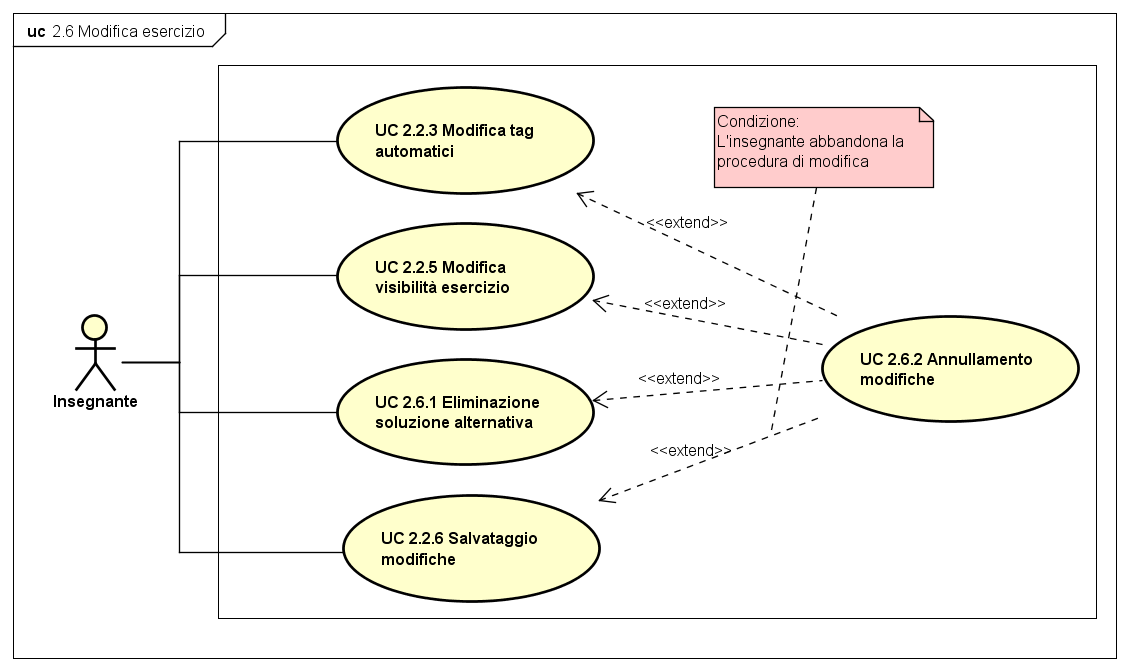
\includegraphics[width=17cm]{img/UC26.png} 
\caption{Caso d'uso UC 2.6}
\end{figure}

\begin{itemize}
	\item[•] \textbf{Attori}: Insegnante;
	\item[•] \textbf{Descrizione}: l’insegnante può modificare il testo, la lingua, la visibilità, i tag e le soluzioni alternative di un esercizio precedentemente inserito;
	\item[•] \textbf{Precondizione}: l'insegnante visualizza lo storico delle frasi inserite;
	\item[•] \textbf{Postcondizione}: l’insegnante ha modificato l'esercizio;
	\item[•] \textbf{Flusso degli eventi}:
		\begin{enumerate}
			\item UC 2.2.5 Modifica tag automatici;
			\item UC 2.2.6 Modifica visibilità esercizio;
			\item UC 2.6.1 Elimina soluzione alternativa;
			\item UC 2.2.8 Salvataggio modifiche.
		\end{enumerate}
	\item[•] \textbf{Estensioni}
	\begin{enumerate}
		\item UC 2.6.2 Annullamento modifiche.
	\end{enumerate}
\end{itemize}   

\subsubsection{UC 2.6.1 Eliminazione soluzione alternativa}
\begin{itemize}
	\item[•] \textbf{Attori}: Insegnante;
	\item[•] \textbf{Descrizione}: l'insegnante elimina una delle soluzioni alternative inserite in precedenza;
	\item[•] \textbf{Precondizione}: l'insegnante sta modificando un esercizio;
	\item[•] \textbf{Postcondizione}: l'insegnante ha eliminato una soluzione alternativa di un esercizio.
	\item[•] \textbf{Flusso degli eventi}: l'insegnante ha iniziato la procedura di modifica esercizio, ha modificato i tag automatici e la visibilità.
\end{itemize}

\subsubsection{UC 2.6.2 Annullamento modifiche}
\begin{itemize}
	\item[•] \textbf{Attori}: Insegnante;
	\item[•] \textbf{Descrizione}: l'insegnante annulla le modifiche inserite all'interno di un esercizio; 
	\item[•] \textbf{Precondizione}: l'insegnante sta modificando un esercizio;
	\item[•] \textbf{Postcondizione}: l'esercizio non è modificato.
	\item[•] \textbf{Flusso degli eventi}: l'insegnante ha iniziato la procedura di modifica esercizio e ha modificato i tag automatici, la visibilità e ha eliminato la soluzione alternativa se è presente.
\end{itemize}

\subsubsection{UC 2.7 Eliminazione esercizio}
\begin{itemize}
	\item[•] \textbf{Attori}: Insegnante;
	\item[•] \textbf{Descrizione}: l'insegnante ha la possibilità di eliminare un esercizio da lei precedentemente inserito;
	\item[•] \textbf{Precondizione}: l'insegnante visualizza lo storico delle frasi inserite;
	\item[•] \textbf{Postcondizione}: l'insegnante ha eliminato l'esercizio precedentemente inserito;
	\item[•] \textbf{Flusso degli eventi}: l'insegnante si è autenticato, si trova nel suo profilo personale e sta visualizzando gli esercizi precedentemente inseriti.
\end{itemize}